\documentclass[chaptersright]{informeutn}
\usepackage[utf8]{inputenc}
\usepackage{array}
\usepackage{geometry}
\usepackage[table]{xcolor}
\usepackage{colortbl}
\usepackage{caption}
\usepackage{graphicx}

\materia{Dispositivos Electronicos I}
\titulo{Trabajo Practico N°2: Diodos rectificadores y zener}
\comision{3R2}
\autores{Documentador y operador: Gaston Grasso 401892\\ Coordinador: Angelo Prieto 401012}
\fecha{27-05-2025}

\begin{document}
\maketitle
\tableofcontents

\chapter{Introduccion}

  El estudio de los diodos rectificadores y zener resulta fundamental para la comprensión y el diseño de circuitos
  electrónicos de potencia y regulación. Estos componentes presentan comportamientos no lineales que deben analizarse
  cuidadosamente, tanto en condiciones normales como en situaciones extremas de funcionamiento. En este trabajo práctico
  se propone un abordaje integral que combina la simulación mediante modelos SPICE con la implementación y medición
  experimental de circuitos sencillos en laboratorio.
    
  Los objetivos principales de esta experiencia son: analizar las especificaciones de los diodos rectificadores y zener,
  identificar su comportamiento en términos de tensión, corriente y disipación de potencia, y evaluar la fidelidad de
  los modelos de simulación ajustando sus parámetros internos en base a los datos provistos por los fabricantes.
  Asimismo, se busca contrastar los resultados obtenidos en simulación con mediciones reales, utilizando instrumentos
  como el multímetro y el osciloscopio, con el fin de comprender las limitaciones prácticas y validar los modelos
  teóricos empleados.

  Este enfoque teórico-práctico permite no solo consolidar conocimientos sobre el funcionamiento de estos dispositivos
  semiconductores, sino también desarrollar habilidades en el uso de herramientas de simulación y medición, esenciales
  para la práctica profesional en ingeniería electrónica.
  
\chapter{Identificacion de pines}

  \begin{center}
  \begin{table}[h!]
  \centering
  \renewcommand{\arraystretch}{2}
  \begin{tabular}{|m{4cm}|>{\centering}m{2cm}|>{\centering}m{2cm}|>{\centering}m{2cm}|>{\centering\arraybackslash}m{2cm}|}
  \hline
  \textbf{Sentido de las puntas del multímetro} & \multicolumn{2}{c|}{\textbf{Diodo de silicio}} & \multicolumn{2}{c|}{\textbf{Diodo de germanio}} \\
  \cline{2-5}
  & D1 & D2 & D1 & D2 \\
  \hline
  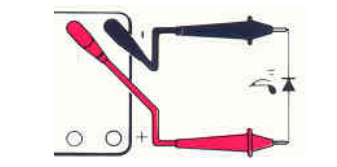
\includegraphics[width=3.5cm]{pictures/polaridad_multimetro1.png} &  &  &  &  \\
  \hline
  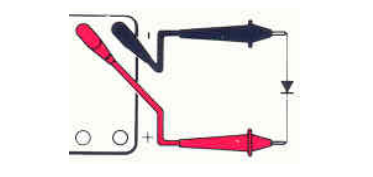
\includegraphics[width=3.5cm]{pictures/polaridad_multimetro2.png} &  &  &  &  \\
  \hline
  \end{tabular}
  \caption{Resultados de las mediciones con el multimetro en modo diodo}
  \end{table}
  \end{center}





\chapter{Curva caracteristica del diodo}

  \section{Actividad de simulación}
  
 
\begin{figure}[h]
  \centering
  \begin{minipage}{0.45\textwidth}
    \centering
    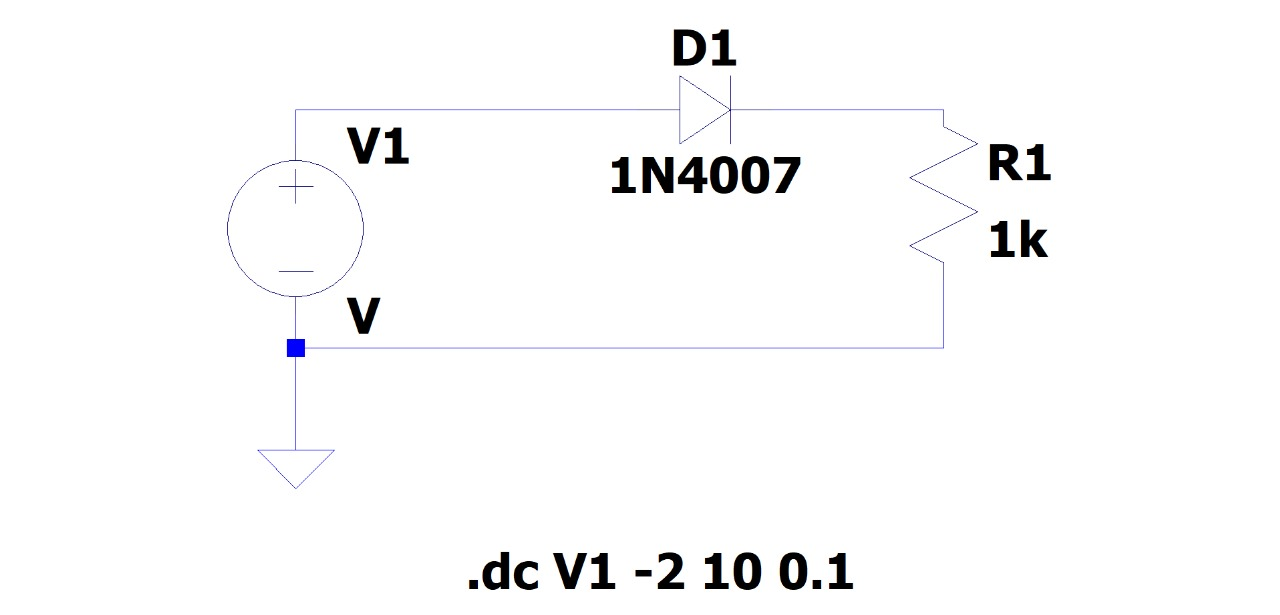
\includegraphics[width=\linewidth]{pictures/curva_diodo_silicio_circuito.jpeg}
    \captionof{figure}{Epígrafe de la primera foto.}
  \end{minipage}
  \hfill
  \begin{minipage}{0.45\textwidth}
    \centering
    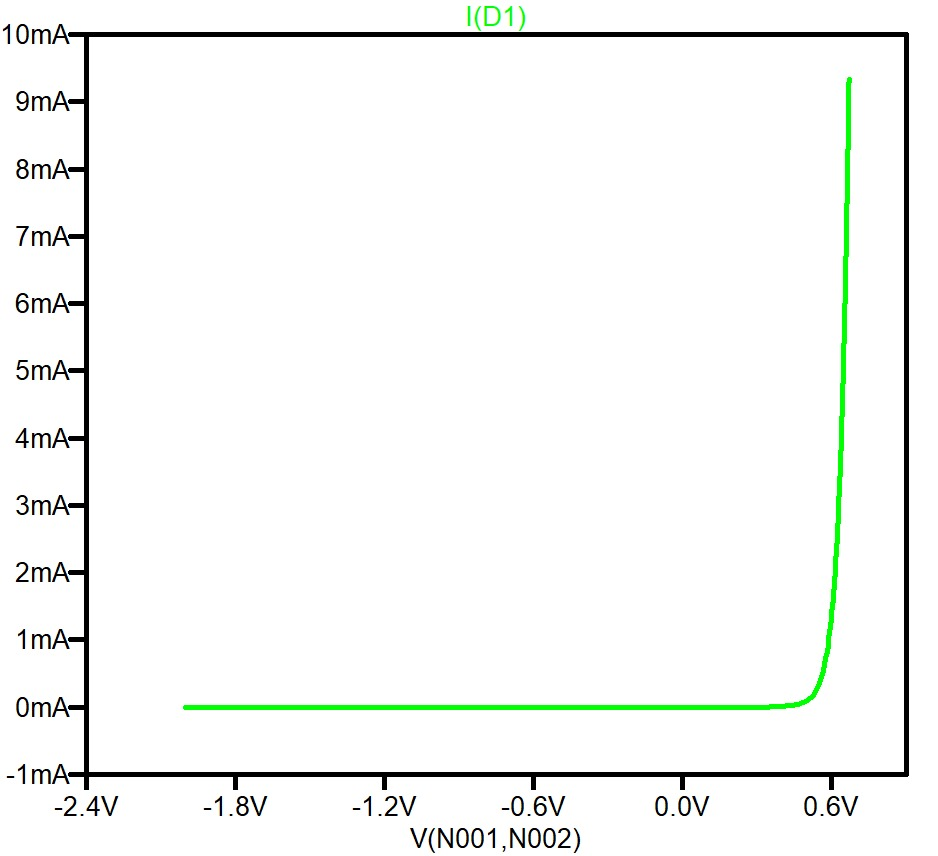
\includegraphics[width=\linewidth]{pictures/curva_diodo_silicio_grafico.jpeg}
    \captionof{figure}{Epígrafe de la segunda foto.}
  \end{minipage}

  \vspace{0.5cm}
  
  \caption{Epígrafe general de las dos imágenes.}
  \label{c}
\end{figure}


\begin{figure}[h]
  \centering
  \begin{minipage}{0.45\textwidth}
    \centering
    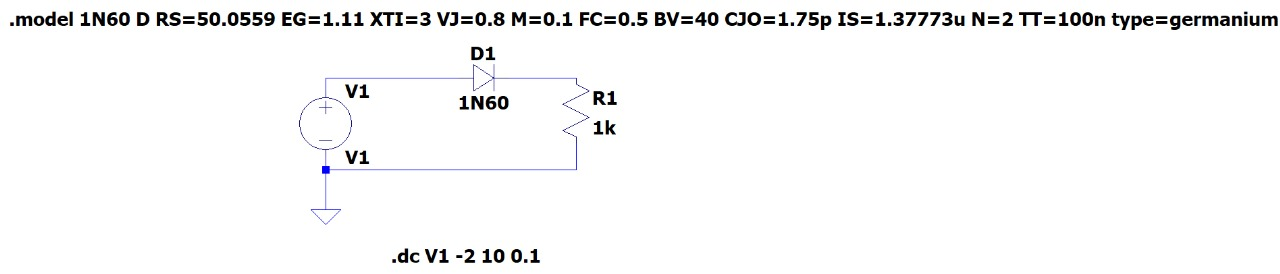
\includegraphics[width=\linewidth]{pictures/curva_diodo_germanio_circuito.jpeg}
    \captionof{figure}{Epígrafe de la primera foto.}
  \end{minipage}
  \hfill
  \begin{minipage}{0.45\textwidth}
    \centering
    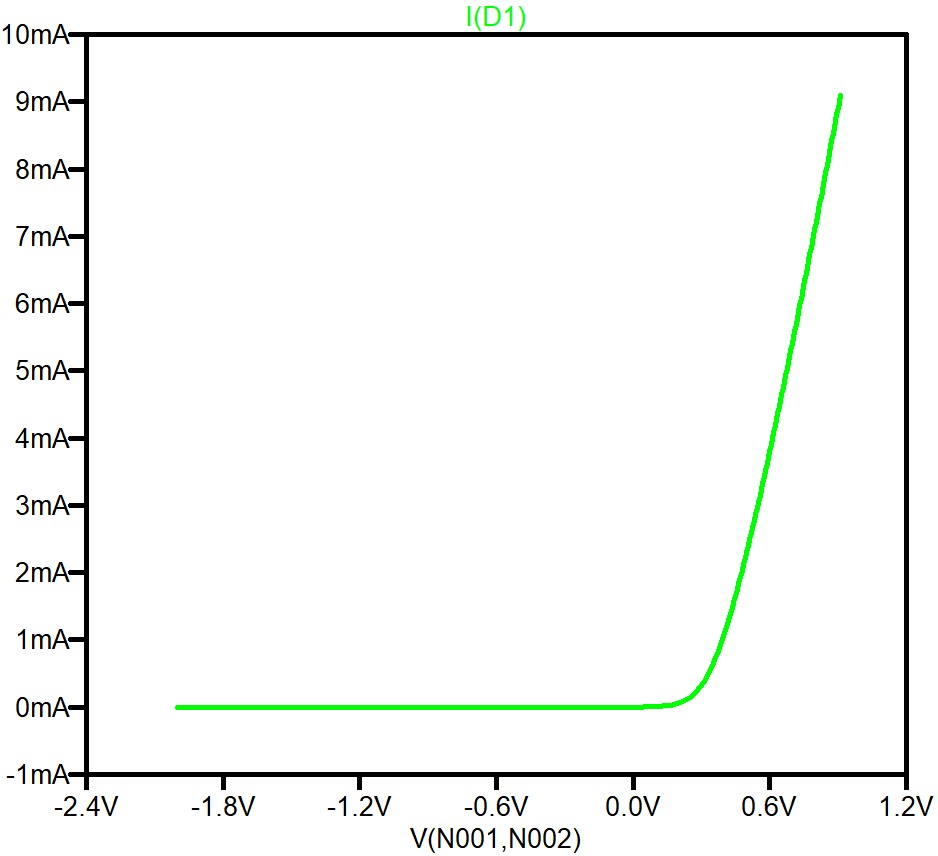
\includegraphics[width=\linewidth]{pictures/curva_diodo_germanio_grafico.jpeg}
    \captionof{figure}{Epígrafe de la segunda foto.}
  \end{minipage}

  \vspace{0.5cm}
  
  \caption{Epígrafe general de las dos imágenes.}
  \label{d}
\end{figure}


\newpage

  \section{Actividad de laboratortio}
    En las clases teóricas se ha visto que el diodo no tiene un comportamiento lineal. Pudimos observar su 
    comportamiento no lineal en la simulación del inciso anterior. Ahora, lo observaremos en el laboratorio de la
    facultad, con el objetivo de comprobar la teoría y la simulación con la realidad. Para lograr esto, implementaremos
    el siguiente circuito:

    \begin{figure}[H]
        \centering
        \begin{tikzpicture}
    	% Paths, nodes and wires:
    	\draw (8.25, 4.5) to[empty diode, l={$D$}, label distance=0.02cm] (8.25, 2.75);
    	\draw (5.25, 4.75) to[american resistor, l={$R_D$}, label distance=0.02cm] (7.25, 4.75);
    	\draw (2.75, 2.75) to[voltmeter, l={$V_{in}$}, label distance=0.02cm] (2.75, 4.5);
    	\draw (9.75, 2.75) to[voltmeter, l_={$V_d$}, label distance=0.02cm] (9.75, 4.5);
    	\draw (5.25, 2.5) to[ammeter, l={$I_D$}, label distance=0.02cm] (7.25, 2.5);
    	\draw (4.25, 4.5) -| (4.25, 4.75) -- (5.25, 4.75);
    	\draw (4.25, 2.75) -| (4.25, 2.5) -- (5.25, 2.5);
    	\draw (7.25, 4.75) -- (8.25, 4.75) -| (8.25, 4.5);
    	\draw (7.25, 2.5) -- (8.25, 2.5) -| (8.25, 2.75);
    	\draw (8.25, 4.75) -- (9.75, 4.75) -| (9.75, 4.5);
    	\draw (8.25, 2.5) -| (9.75, 2.75);
    	\draw (2.75, 4.5) -| (2.75, 4.75) -- (4.25, 4.75);
    	\draw (2.75, 2.75) -| (2.75, 2.5) -- (4.25, 2.5);
    	\draw (4.25, 4.5) to[battery1, l={$V$}, label distance=0.02cm] (4.25, 2.75);
        \end{tikzpicture}
        \caption{\footnotesize
        Circuito básico del diodo en polarización directa con los instrumentos de medición.}
    \end{figure}

    En este circuito, $V$ es una fuente de tensión variable, con la cual alimentaremos el circuito para analizar el 
    comportamiento del diodo en varios puntos y así poder trazar una curva de características del mismo. Se han tomado
    10 puntos, partiendo de 0V hasta 5V.
    
    A continuación, se presenta una tabla, tanto para el diodo de $Si$ como para el de $Ge$, con los valores obtenidos 
    de $V_D$ e $I_D$ para los distintos valores de alimentación. También, se presenta una gráfica de las curvas de 
    características obtenidas para ambos diodos y, fotografías de los instrumentos de medición utilizados y disposición 
    de los circuitos:
  
    \subsubsection{Diodo de silicio}
    
      \begin{table}[H]
      \centering 
      \renewcommand{\arraystretch}{1.5}
      \setlength{\tabcolsep}{8pt}
      \resizebox{\textwidth}{!}{
      \begin{tabular}{|c|*{13}{c|}}
      \hline
      \textbf{$V_1$ [V]} & 0 & 0.098 & 0.304 & 0.399 & \cellcolor{yellow}0.448 & \cellcolor{yellow}0.491 & \cellcolor{yellow}0.548 & \cellcolor{yellow}0.599 & \cellcolor{yellow}0.653 & \cellcolor{yellow}0.693 & 1.047 & 3.028 & 5.037 \\
      \hline
      $V_D[V]$ & 0 & 0.097 & 0.29 & 0.37 & 0.4 & 0.42 & 0.44 & 0.46 & 0.48 & 0.48 & 0.53 & 0.61 & 0.64 \\
      \hline
      $I_D[mA]$ & 0 & 0 & 0 & 0 & 0 & 0.053 & 0.087 & 0.124 & 0.165 & 0.196 & 0.511 & 2.4 & 4.4 \\
      \hline
      \end{tabular}
      }
      \caption{Tabla de valores $V_D$ e $I_D$ para diodo de silicio 1N4007.}
      \label{a}
      \end{table}
    
    \subsubsection{Diodo de germanio}
      \begin{table}[H]
      \centering
      \renewcommand{\arraystretch}{1.5}
      \setlength{\tabcolsep}{8pt}
      \resizebox{\textwidth}{!}{
      \begin{tabular}{|c|*{13}{c|}}
      \hline
      \textbf{$V_1$ [V]} & 0.051 & 0.103 & 0.154 & 0.201 & \cellcolor{yellow}0.245 & \cellcolor{yellow}0.301 & \cellcolor{yellow}0.344 & \cellcolor{yellow}0.674 & \cellcolor{yellow}0.694 & \cellcolor{yellow}0.907 & 1.5 & 3 & 5 \\
      \hline
      $V_D[V]$ & 0.04 & 0.08 & 0.13 & 0.16 & 0.18 & 0.19 & 0.22 & 0.26 & 0.24 & 0.26 & 0.28 & 0.32 & 0.35 \\
      \hline
      $I_D[mA]$ & 0.0006 & 0.0027 & 0.012 & 0.029 & 0.055 & 0.1 & 0.19 & 0.68 & 0.4 & 0.6 & 1.2 & 2.7 & 4.7 \\
      \hline
      \end{tabular}
      }
      \caption{Tabla de valores $V_D$ e $I_D$ para diodo de germanio 1N60.}
      \label{b}
      \end{table}

    \subsubsection{Curvas $I_D$ vs $V_D$}
    \begin{figure}[H]
        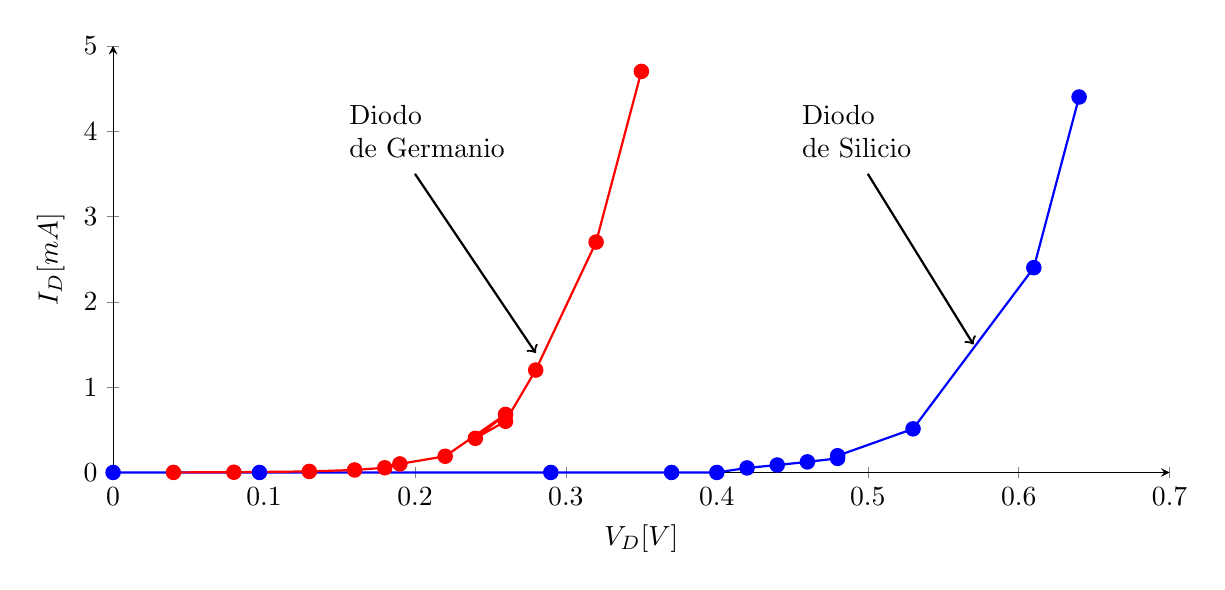
\begin{tikzpicture}
          \begin{axis}[
            axis lines = left,
            ylabel = {$I_{D}[mA]$},
            xlabel = {$V_{D}[V]$},
            width=15cm,
            height=7cm,
            ymin=0, ymax=5,
            xmin=0, xmax=0.7,
            ytick={0,1,2,3,4,5},
            xtick={0,0.1,0.2,0.3,0.4,0.5,0.6,0.7},
            clip=false, % necesario para dibujar fuera del área del gráfico
          ]
            % DIODO SILICIO
            \addplot[
              color=blue,
              mark=*,
              only marks,
              mark options={scale=1.3}
            ]
            coordinates {
                (0, 0)
                (0.097, 0)
                (0.29, 0)
                (0.37, 0)
                (0.4, 0)
                (0.42, 0.053)
                (0.44, 0.087)
                (0.46, 0.124)
                (0.48, 0.165)
                (0.48, 0.196)
                (0.53, 0.511)
                (0.61, 2.4)
                (0.64, 4.4)
            };
            \addplot[
              color=blue,
              thick
            ]
            coordinates {
                (0, 0)
                (0.097, 0)
                (0.29, 0)
                (0.37, 0)
                (0.4, 0)
                (0.42, 0.053)
                (0.44, 0.087)
                (0.46, 0.124)
                (0.48, 0.165)
                (0.48, 0.196)
                (0.53, 0.511)
                (0.61, 2.4)
                (0.64, 4.4)
            };
            \node[align=left, anchor=west] at (axis cs:0.45,4) {Diodo\\de Silicio};
            \draw[->, thick] (axis cs:0.5,3.5) -- (axis cs:0.57,1.5);
            % FIN DIODO SILICIO
            % DIODO GERMANIO
            \addplot[
              color=red,
              mark=*,
              only marks,
              mark options={scale=1.3}
            ]
            coordinates {
                (0.04, 0.0006)
                (0.08, 0.0027)
                (0.13, 0.012)
                (0.16, 0.029)
                (0.18, 0.055)
                (0.19, 0.1)
                (0.22, 0.19)
                (0.26, 0.68)
                (0.24, 0.4)
                (0.26, 0.6)
                (0.28, 1.2)
                (0.32, 2.7)
                (0.35, 4.7)
            };
            \addplot[
              color=red,
              thick
            ]
            coordinates {
                (0.04, 0.0006)
                (0.08, 0.0027)
                (0.13, 0.012)
                (0.16, 0.029)
                (0.18, 0.055)
                (0.19, 0.1)
                (0.22, 0.19)
                (0.26, 0.68)
                (0.24, 0.4)
                (0.26, 0.6)
                (0.28, 1.2)
                (0.32, 2.7)
                (0.35, 4.7)
            };
            \node[align=left, anchor=west] at (axis cs:0.15,4) {Diodo\\de Germanio};
            \draw[->, thick] (axis cs:0.2,3.5) -- (axis cs:0.28,1.4);
            % FIN DIODO GERMANIO
          \end{axis}
        \end{tikzpicture}
        \caption{\footnotesize
        Gráfica con las curvas $I_D$ vs $V_D$ (medidos en el laboratorio) de los diodos de Silicio y Germanio.}
        \end{figure}
      
    \subsubsection{Fotografías}
      \begin{figure}[H]
        \centering
        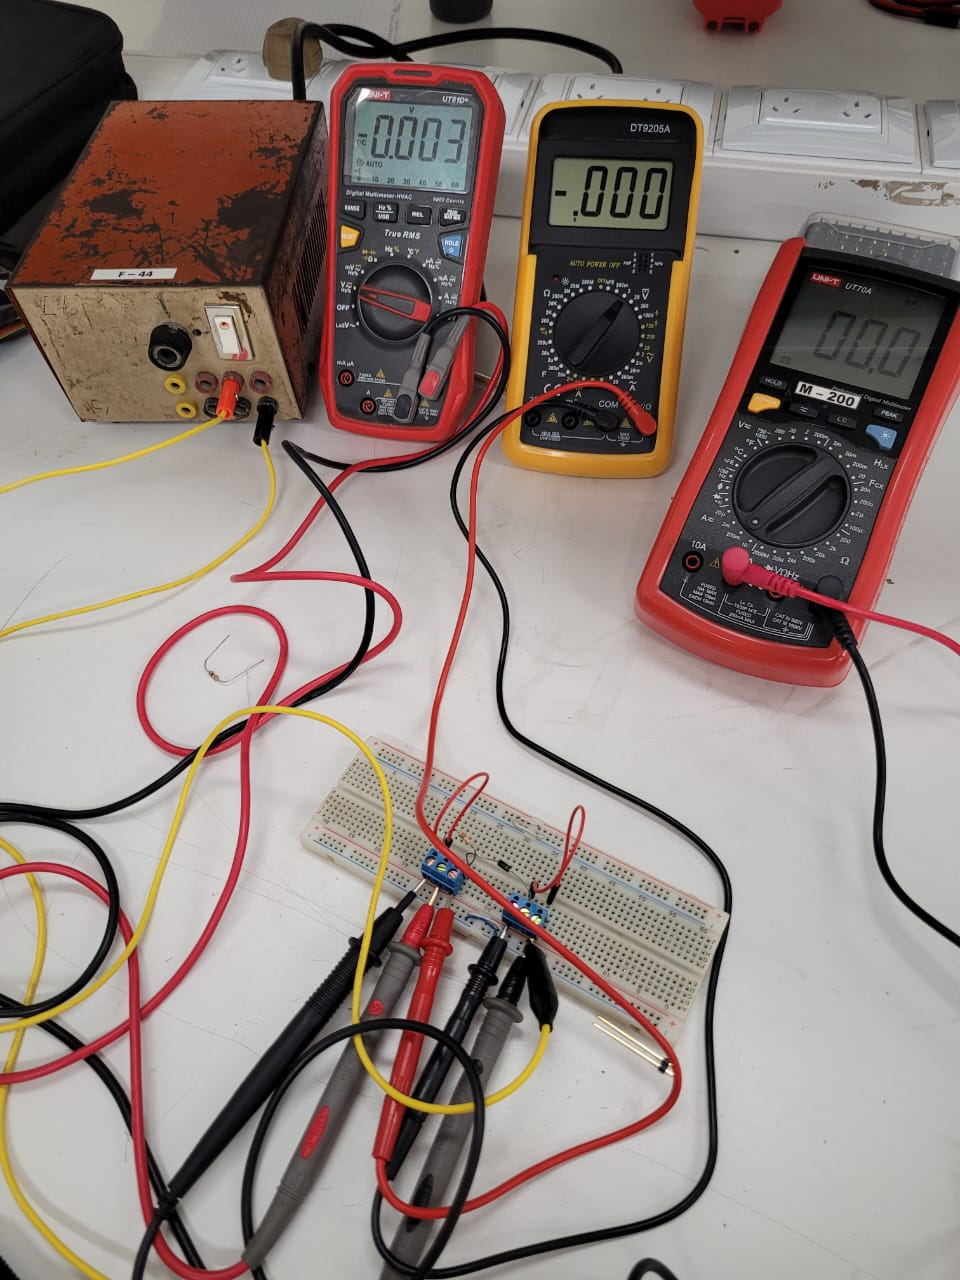
\includegraphics[width=.35\textwidth]{pictures/disposicion-elementos.jpeg}
        \caption{Fotografía general de los elementos utilizados para los ensayos.}
      \end{figure}
      \begin{figure}[h!]
        \centering
        \begin{minipage}{0.40\textwidth}
            \centering
            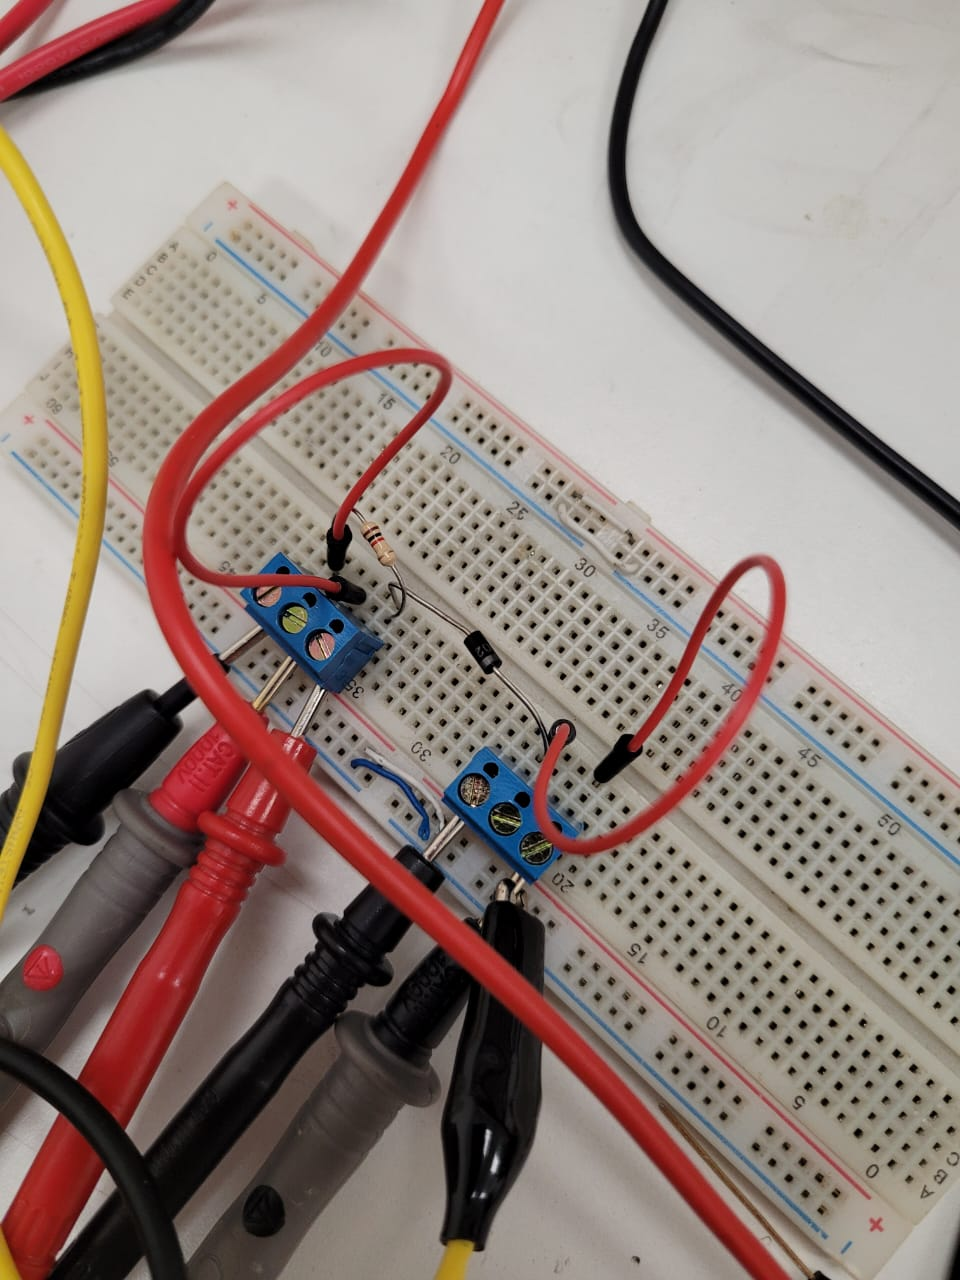
\includegraphics[width=\textwidth]{pictures/disposicion-circuito-silicio.jpeg}
            \caption{Disposición de los elementos del circuito. Diodo de Silicio.}
            \label{fig:silicio}
        \end{minipage}
        \hspace{0.05\textwidth} % Espacio entre imágenes
        \begin{minipage}{0.5\textwidth}
            \centering
            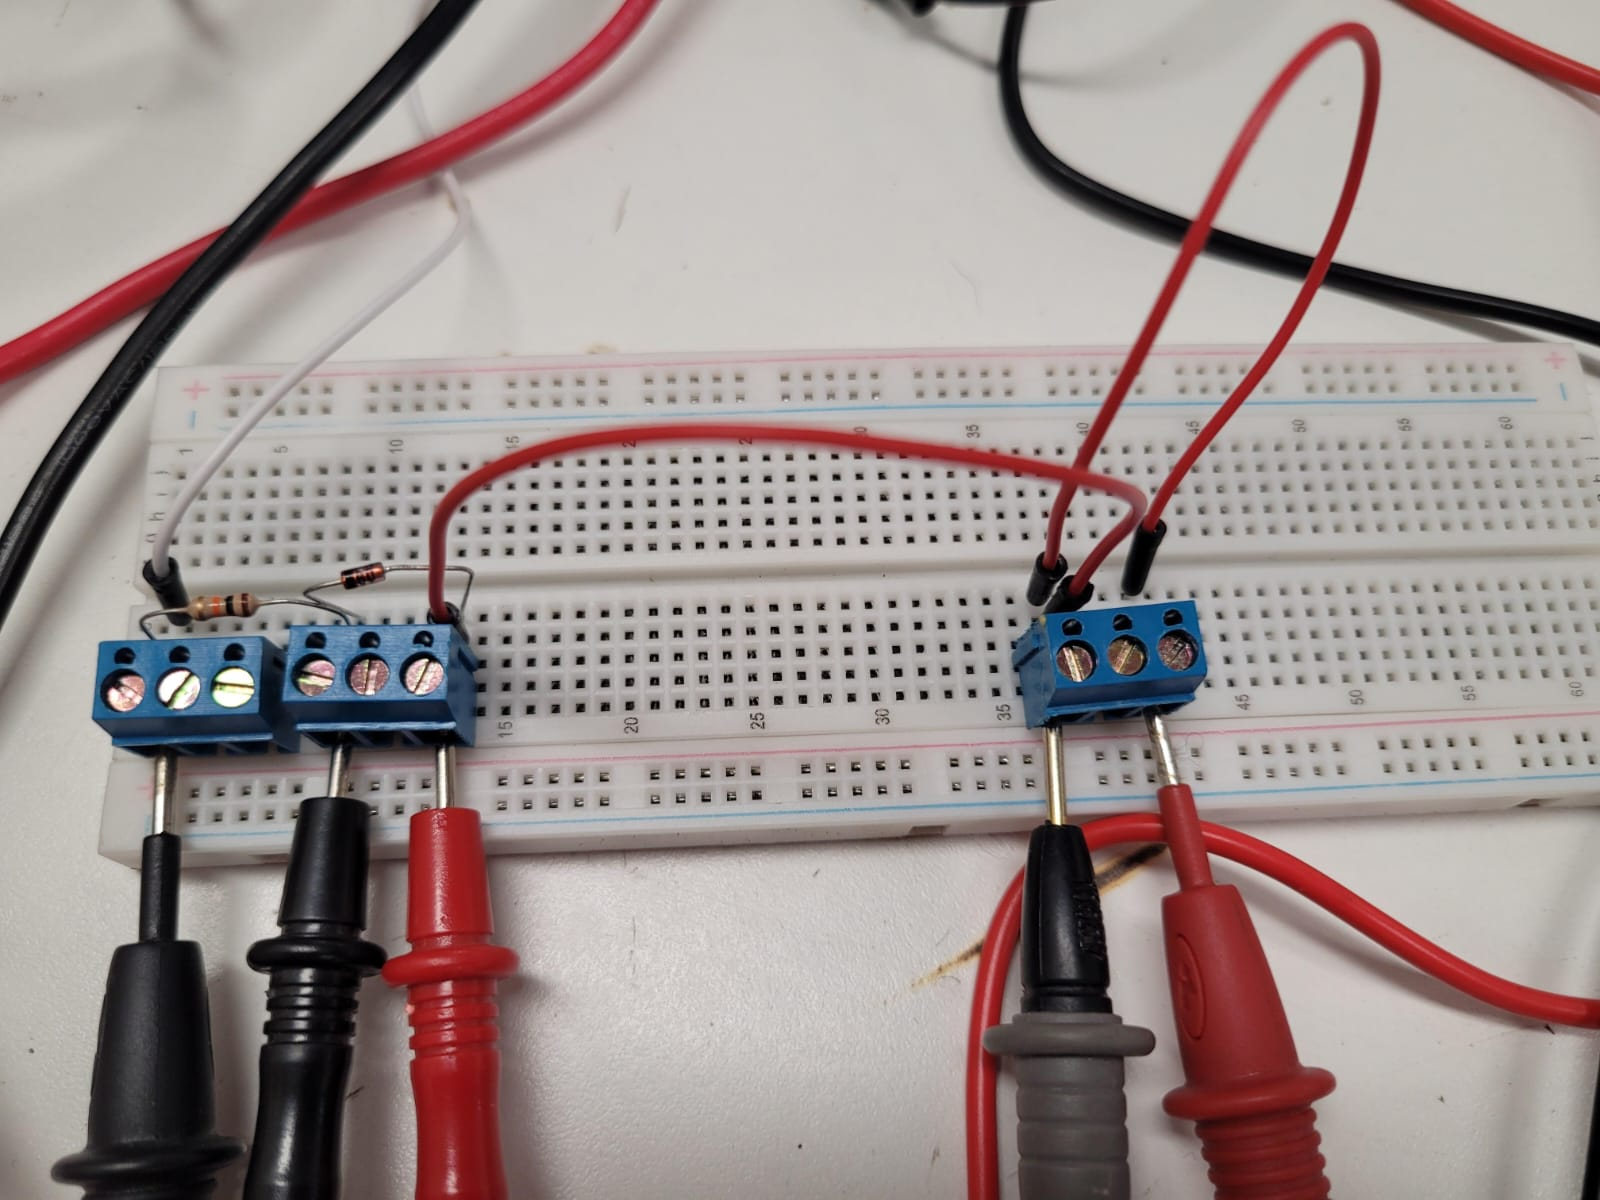
\includegraphics[width=\textwidth]{pictures/disposicion-circuito-germanio.jpeg}
            \caption{Disposición de los elementos del circuito. Diodo de Germanio.}
            \label{fig:germanio}
        \end{minipage}
    \end{figure}
    \begin{figure}[h!]
        \centering
        \begin{minipage}{0.3\textwidth}
            \centering
            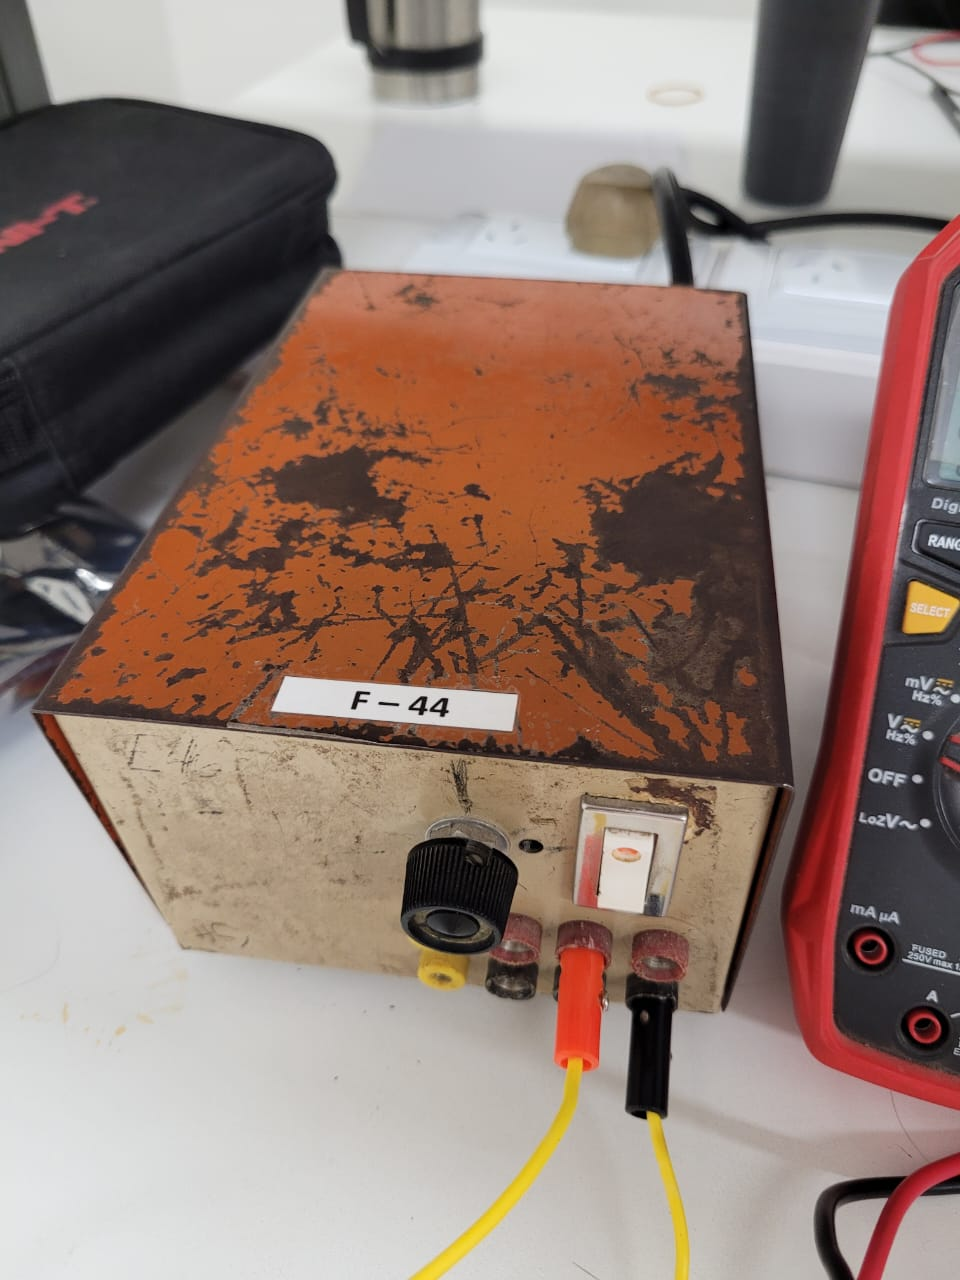
\includegraphics[width=\textwidth]{pictures/fuentealim.jpeg}
            \caption{Instrumentos: fuente de alimentación proporcionado por el laboratorio.}
        \end{minipage}
        \hspace{0.05\textwidth} % Espacio entre imágenes
        \begin{minipage}{0.3\textwidth}
            \centering
            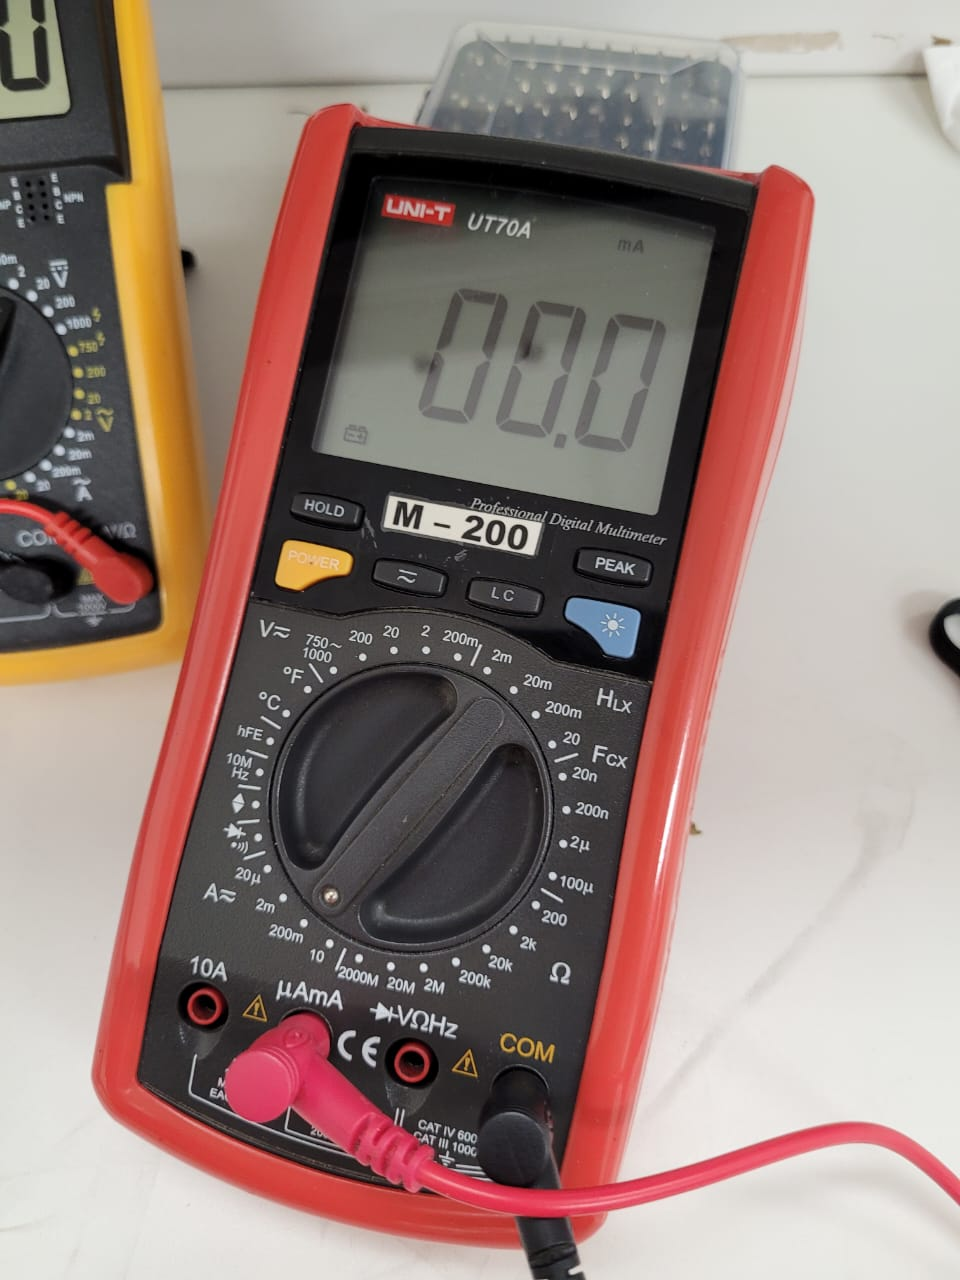
\includegraphics[width=\textwidth]{pictures/multimetro-facu.jpeg}
            \caption{Instrumentos: multimétro digital Nº1, proporcionado por el laboratorio.}
        \end{minipage}
    \end{figure}
    \begin{figure}[h!]
        \centering
        \begin{minipage}{0.3\textwidth}
            \centering
            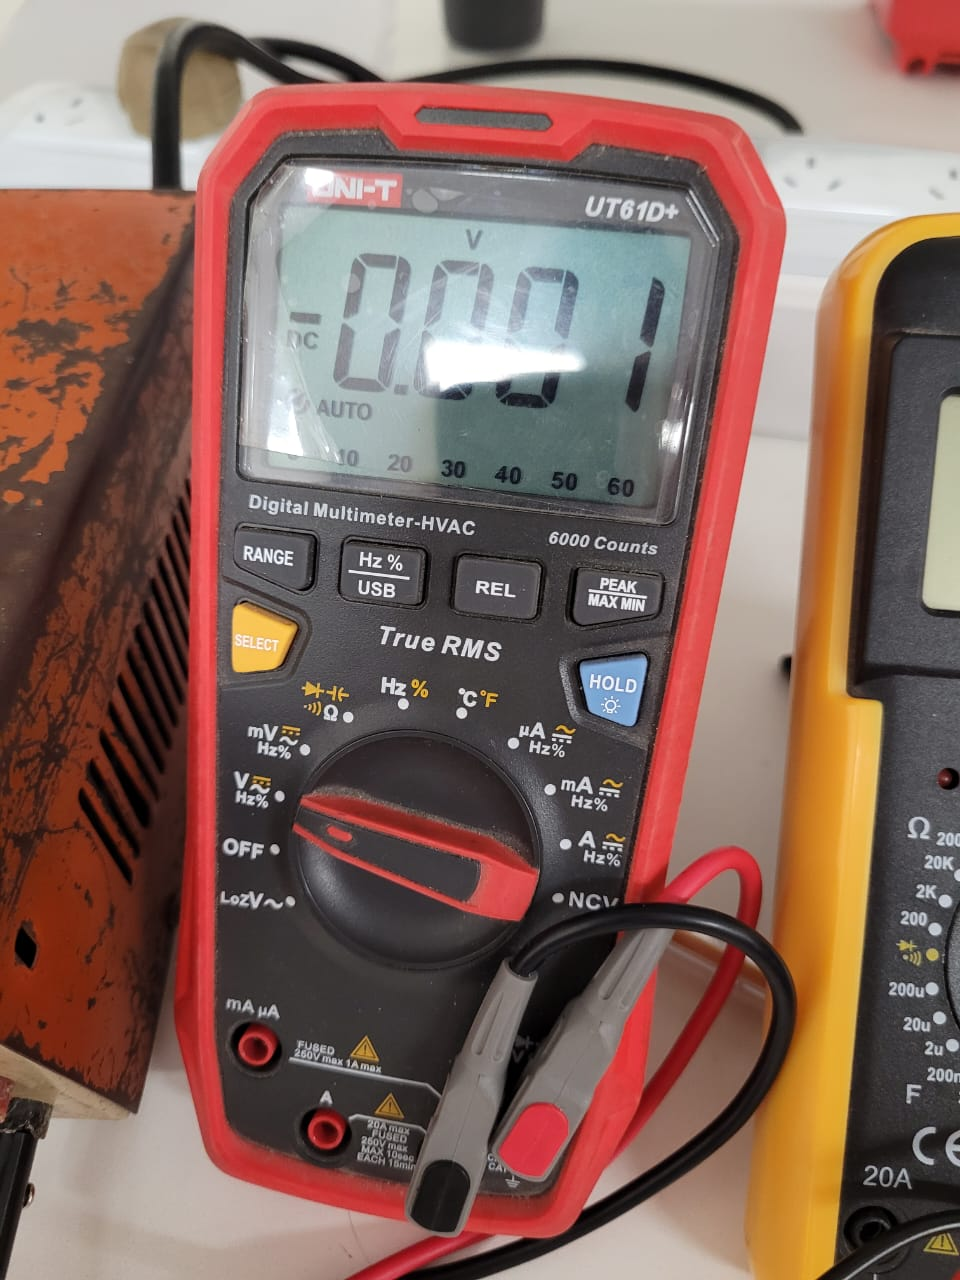
\includegraphics[width=\textwidth]{pictures/multimetro-gaston.jpeg}
            \caption{Instrumentos: multimétro digital Nº2.}
        \end{minipage}
        \hspace{0.05\textwidth} % Espacio entre imágenes
        \begin{minipage}{0.3\textwidth}
            \centering
            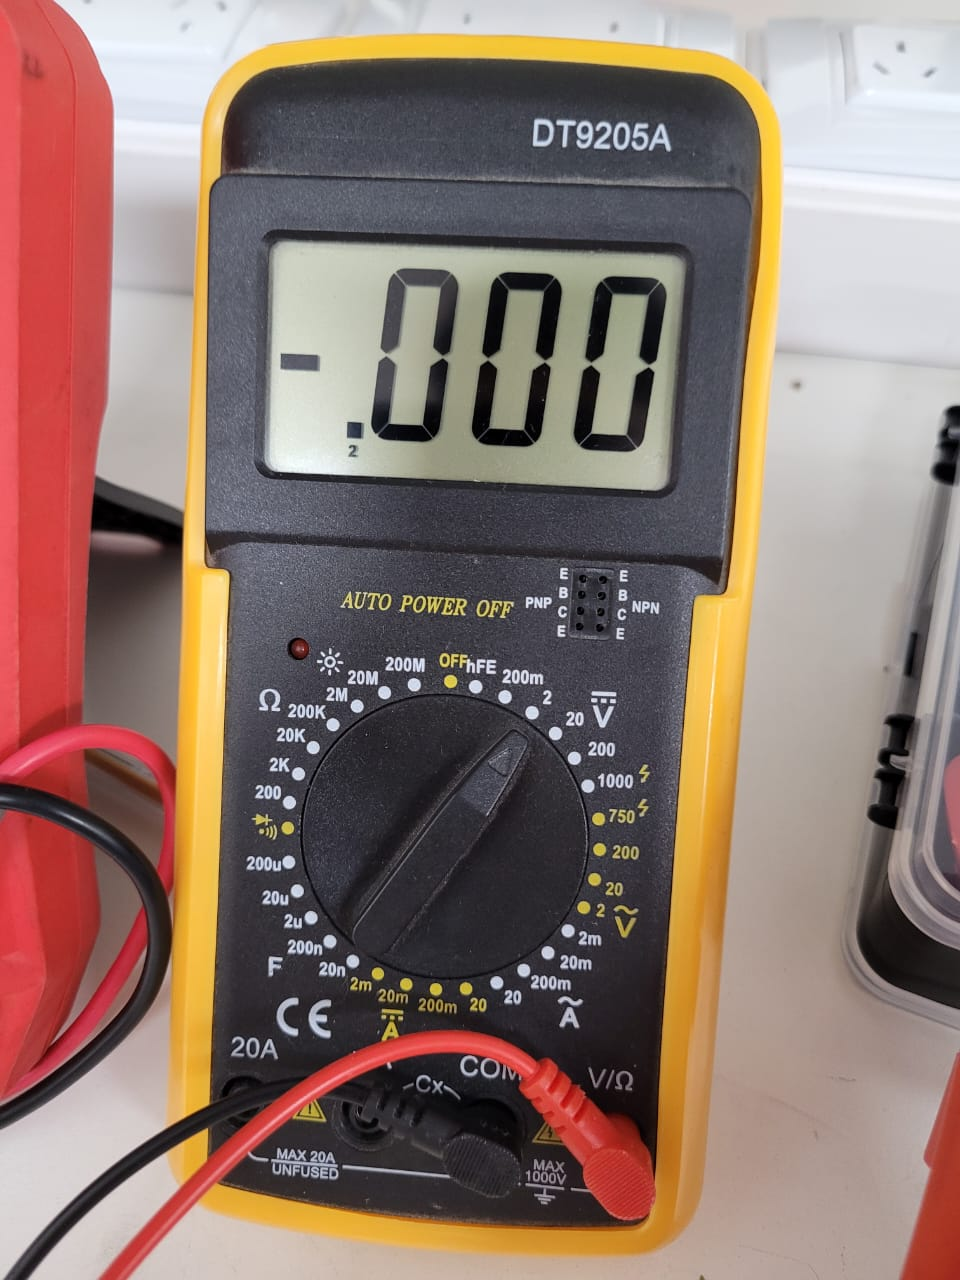
\includegraphics[width=\textwidth]{pictures/multimetro-angelo.jpeg}
            \caption{Instrumentos: multimétro digital Nº3.}
        \end{minipage}
    \end{figure}
    

\chapter{Comportamiento del diodo en función de la temperatura}

  El comportamiento eléctrico de los diodos semiconductores está fuertemente influenciado por la temperatura. Esto se
  debe a la dependencia de parámetros clave del dispositivo con respecto a la temperatura, como la corriente de saturación 
  inversa (\(I_S\)) y la tensión umbral de conducción directa.
  
  \section{Fundamento teórico}
  
    La ecuación característica de un diodo ideal es:
    
    \[
    I_D = I_S \left( e^{\frac{V_D}{n V_T}} - 1 \right)
    \]
    
    donde:
    \begin{itemize}
        \item \(I_D\) es la corriente que circula por el diodo,
        \item \(I_S\) es la corriente de saturación inversa,
        \item \(V_D\) es la tensión aplicada al diodo,
        \item \(n\) es el coeficiente de idealidad (típicamente entre 1 y 2),
        \item \(V_T = \frac{kT}{q}\) es la tensión térmica, que depende linealmente de la temperatura absoluta \(T\), con
            \(k\) siendo la constante de Boltzmann y \(q\) la carga del electrón.
    \end{itemize}
    
    A medida que la temperatura aumenta:
    \begin{enumerate}
        \item El valor de \(V_T\) también aumenta, lo cual afecta la pendiente de la curva \(I\)-\(V\).
        \item La corriente de saturación inversa \(I_S\) se incrementa exponencialmente con la temperatura, dado que 
            depende del número de portadores minoritarios generados térmicamente.
        \item Como consecuencia, la corriente para un mismo voltaje directo es mayor a temperaturas más altas.
        \item La tensión de umbral para que el diodo comience a conducir disminuye.
    \end{enumerate}
  
  \section{Simulación y análisis}
  
    Para observar este efecto, se ha realizado una simulación del diodo 1N3198 sometido a tres temperaturas distintas: 
    20 °C, 100 °C y 125 °C. El circuito simulado se muestra a continuación:
    
    \begin{figure}[H]
        \centering
        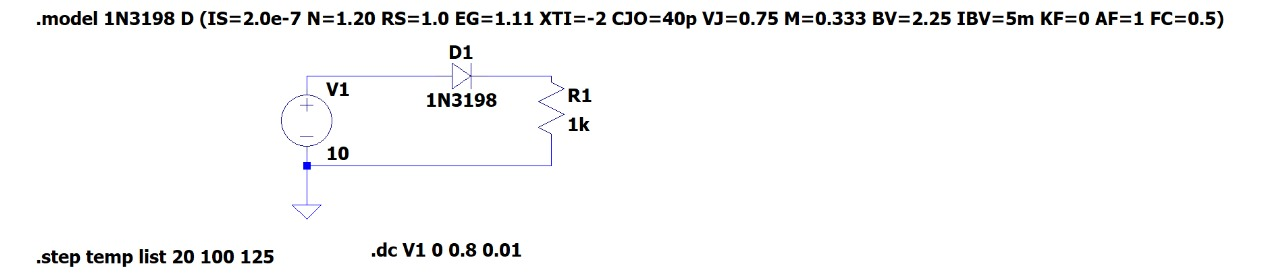
\includegraphics[width=0.7\textwidth]{pictures/comparacion_temperatura_circuito.jpeg}
        \caption{Circuito simulado para análisis de comportamiento térmico del diodo.}
    \end{figure}
    
    En la siguiente gráfica se puede observar cómo varía la curva característica corriente-voltaje del diodo en función de
    la temperatura:
    
    \begin{figure}[H]
        \centering
        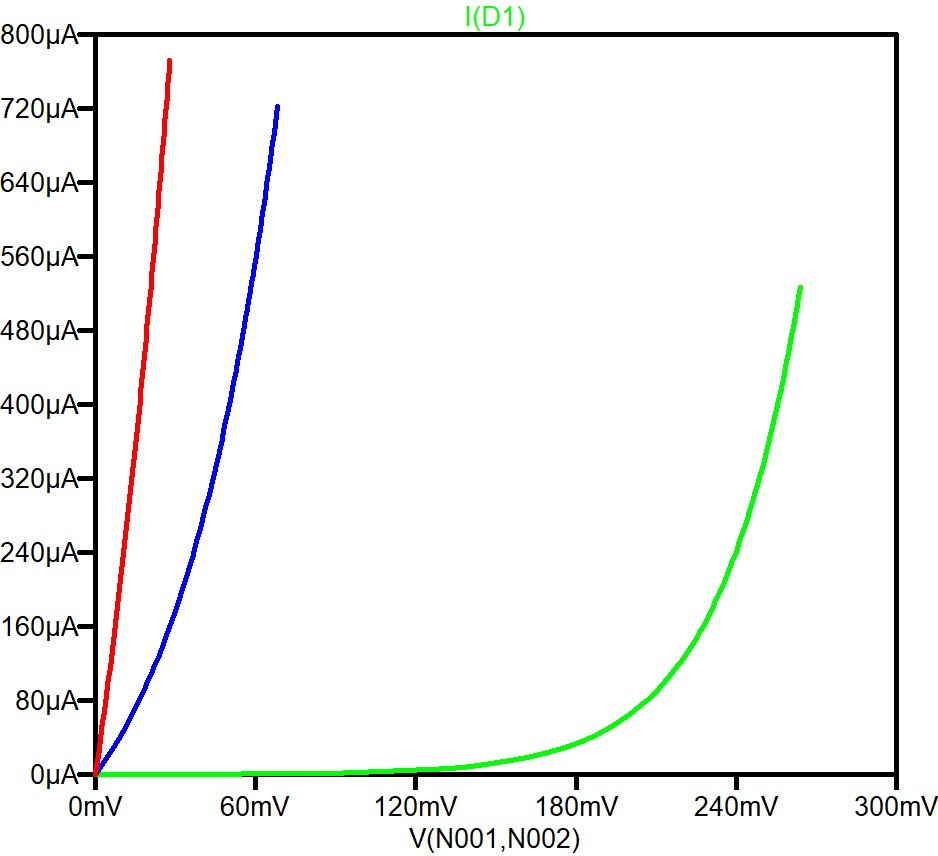
\includegraphics[width=0.7\textwidth]{pictures/comparacion_temperatura_grafico.jpeg}
        \caption{Curvas I-V del diodo 1N3198 a diferentes temperaturas.}
    \end{figure}
    
    Como se puede apreciar, a mayor temperatura, la curva se desplaza hacia la izquierda, lo que indica que el diodo
    comienza a conducir a un menor voltaje. Además, para una misma tensión, la corriente que circula por el diodo es
    considerablemente mayor a temperaturas elevadas. Esta característica es clave en el diseño de circuitos electrónicos, 
    ya que una mala gestión térmica puede provocar corrientes excesivas no deseadas o incluso la destrucción del componente.


\chapter{Circuitos recortadores con diodos zener}

\section{Actividad de simulación}

\subsection*{Circuito a: Regulador de Voltaje con Zener}

\begin{itemize}
    \item \textbf{Objetivo:} Analizar el comportamiento de un circuito con diodo Zener como regulador de voltaje.
    \item \textbf{Simulación:} Se varía el voltaje de entrada \( V_{\text{in}} \) y se observa el comportamiento de la tensión de salida \( V_{\text{out}} \).
\end{itemize}

\subsubsection*{Esquema del circuito}
\begin{center}
    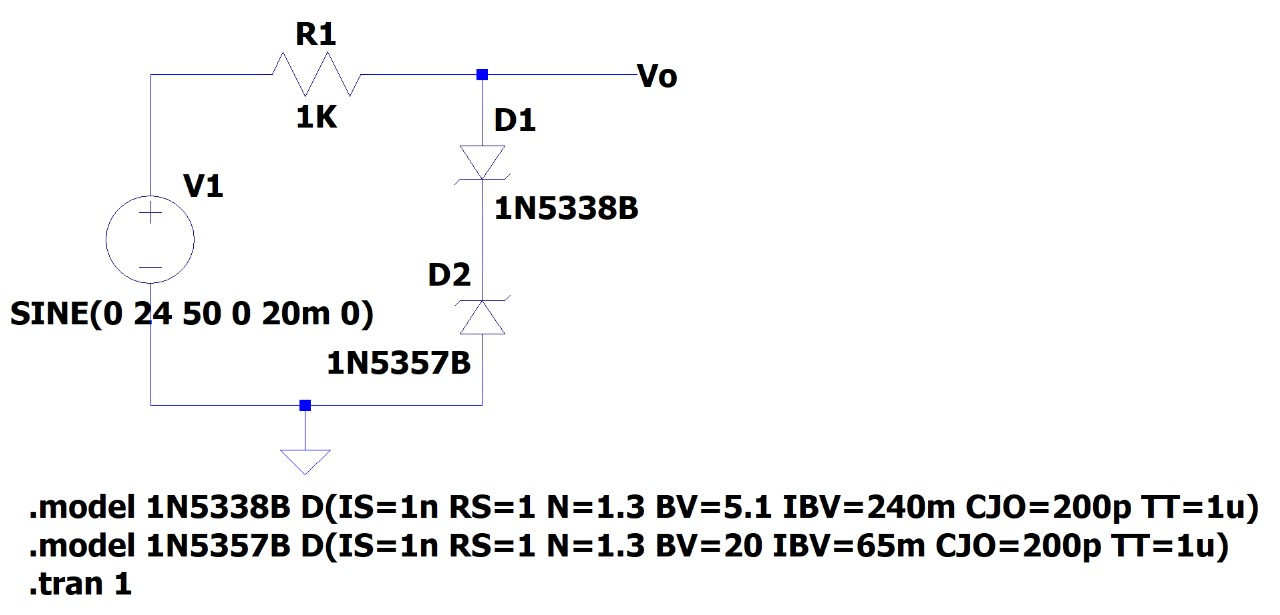
\includegraphics[width=0.5\textwidth]{pictures/zener_1_circuito.jpeg}
\end{center}

\subsubsection*{Análisis del comportamiento}

El diodo Zener se polariza en inversa. Su función principal es mantener la tensión de salida constante mientras el voltaje de entrada sea mayor que su tensión de ruptura \( V_Z \).

\begin{itemize}
    \item Si \( V_{\text{in}} < V_Z \), el diodo no conduce y \( V_{\text{out}} \approx V_{\text{in}} \).
    \item Si \( V_{\text{in}} \geq V_Z \), el diodo entra en conducción inversa (zona Zener) y mantiene \( V_{\text{out}} \approx V_Z \).
\end{itemize}

La corriente que circula por el diodo es:

\[
I_Z = \frac{V_{\text{in}} - V_Z}{R_s}
\]

\subsubsection*{Gráfico de simulación}
\begin{center}
    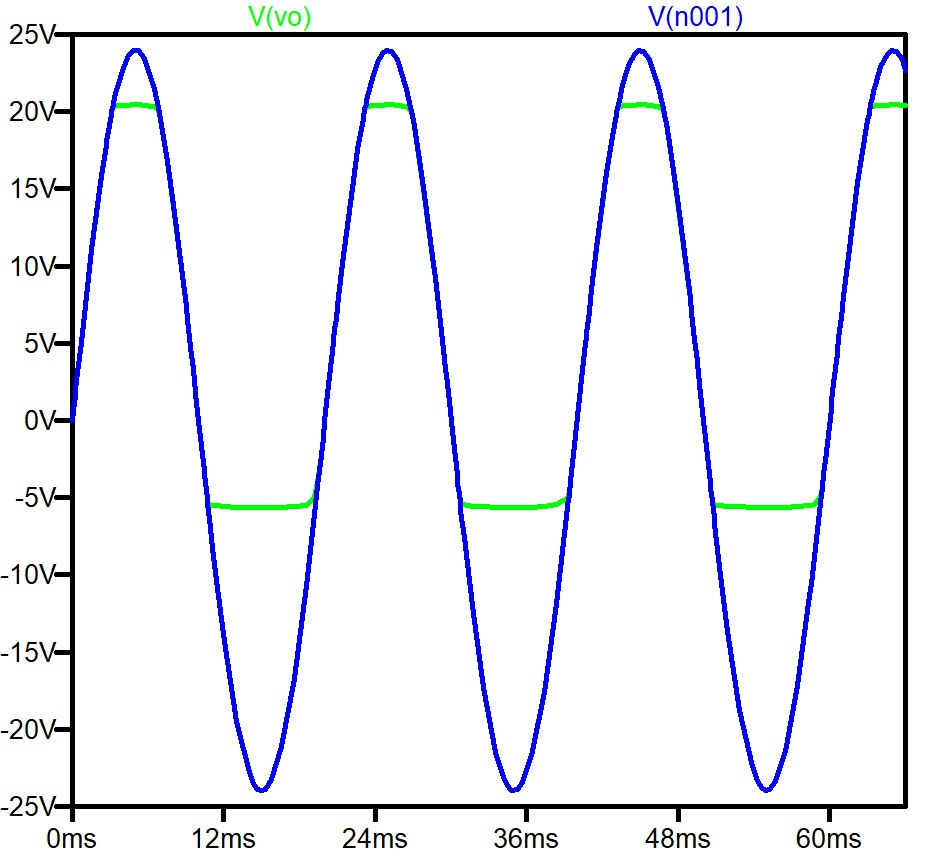
\includegraphics[width=0.6\textwidth]{pictures/zener_1_grafico.jpeg}
\end{center}

\noindent
El gráfico muestra cómo, a partir de cierta tensión, la salida se estabiliza en \( V_Z \), actuando como un recortador superior.


\subsection*{Circuito b: Recortador con Zener de diferente valor}

\begin{itemize}
    \item \textbf{Objetivo:} Observar el efecto de usar un diodo Zener con distinta tensión de ruptura.
\end{itemize}

\subsubsection*{Esquema del circuito}
\begin{center}
    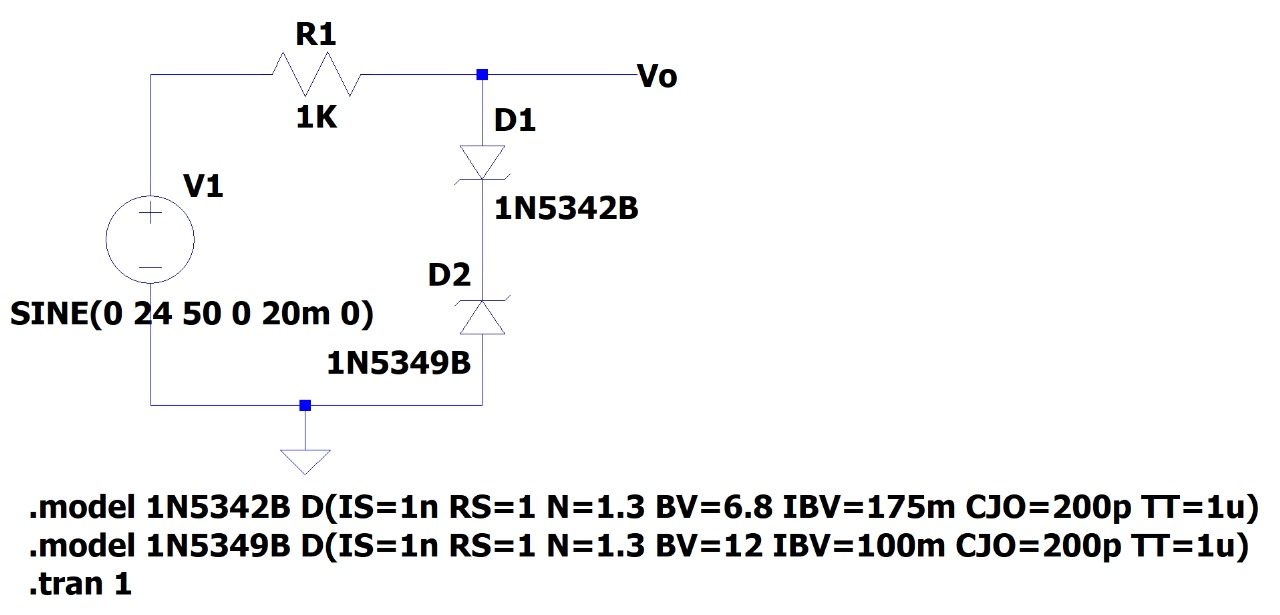
\includegraphics[width=0.5\textwidth]{pictures/zener_2_circuito.jpeg}
\end{center}

\subsubsection*{Análisis del comportamiento}

El principio de funcionamiento es el mismo que en el circuito anterior, pero se utiliza un diodo Zener con otra tensión de ruptura. El voltaje de salida se regula al nuevo valor \( V_Z' \).

\[
V_{\text{out}} =
\begin{cases}
    V_{\text{in}} & \text{si } V_{\text{in}} < V_Z' \\
    V_Z' & \text{si } V_{\text{in}} \geq V_Z'
\end{cases}
\]

\subsubsection*{Gráfico de simulación}
\begin{center}
    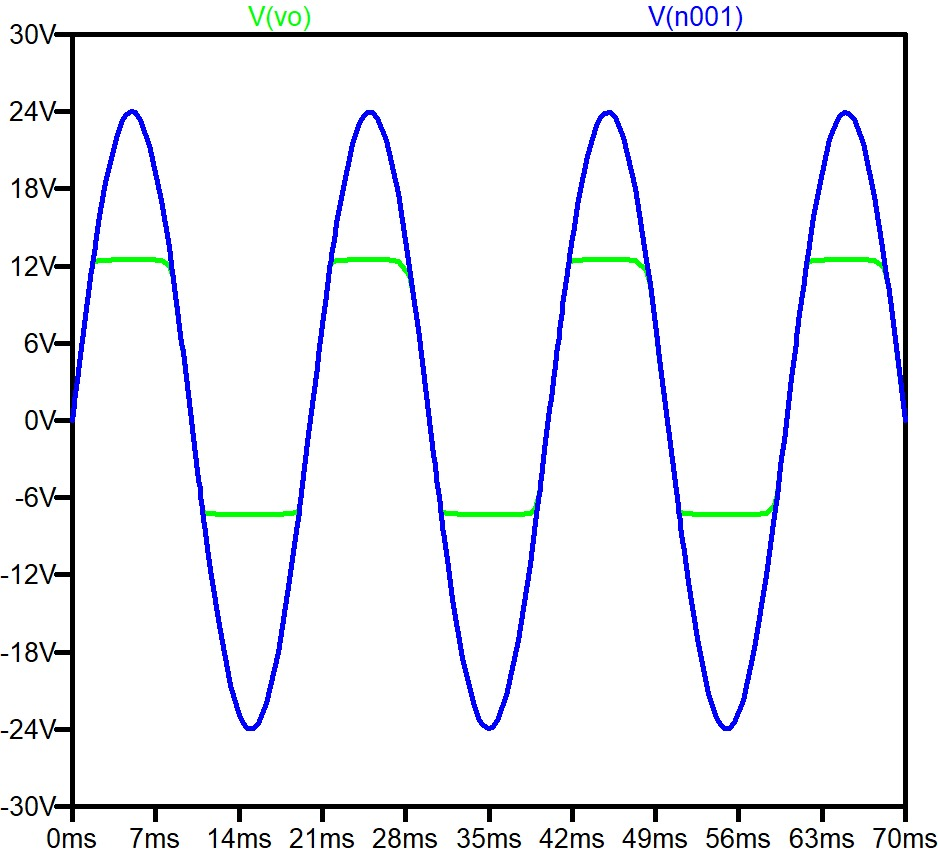
\includegraphics[width=0.6\textwidth]{pictures/zener_2_grafico.jpeg}
\end{center}

\noindent
Se observa un comportamiento similar, con la salida limitada a \( V_Z' \), actuando como recortador, pero en este caso con un umbral de corte distinto.

\section*{Conclusión}

Se comprobó que los diodos Zener permiten recortar el voltaje de salida una vez superado su valor de ruptura. Esto es útil para limitar la tensión en circuitos sensibles, estabilizar señales o implementar fuentes de voltaje fijo. Variar el tipo de diodo Zener modifica el umbral de recorte.


  
  \section{Actividad de laboratortio}

\chapter{Análisis sobre parámetros de hoja de datos}

  \section*{Características Eléctricas}
  
    \subsection*{Regímenes máximos}
      \begin{enumerate}
        \item $V_{RRM}$: Tensión repetitiva máxima en inversa. Es el máximo voltaje que se puede aplicar en polarización inversa de manera repetitiva sin dañar el dispositivo.
        \item $V_{RSM}$: Tensión máxima en inversa no repetitiva. Es el valor pico máximo que puede soportar el dispositivo en condiciones excepcionales.
        \item $I_{FRMS}$: Corriente eficaz directa máxima. Es la corriente RMS que el dispositivo puede conducir de forma continua sin sobrecalentamiento.
        \item $I_{FSM}$: Corriente de sobrecarga directa máxima. Es el valor pico máximo de corriente directa que puede soportar durante un pulso corto.
      \end{enumerate}
    
    \subsection*{Regímenes característicos}
      \begin{enumerate}
        \item $V_{BR}$: Tensión de ruptura. Es el voltaje en el cual el dispositivo comienza a conducir en inversa.
        \item $I_R$: Corriente de fuga inversa. Es la pequeña corriente que circula en inversa antes de la ruptura.
        \item $V_F$: Tensión de conducción directa. Es la caída de tensión directa cuando el dispositivo está conduciendo.
        \item $I_{RM}$: Corriente máxima en inversa. Es la máxima corriente que puede circular en polarización inversa antes de entrar en ruptura.
        \item $I_F$: Corriente directa. Es la corriente que circula a través del dispositivo cuando está polarizado en directa.
      \end{enumerate}
  
  \section*{Características Térmicas}
  
    \begin{enumerate}
        \item $T_J$: Temperatura de unión máxima. Es la temperatura máxima permitida en la unión del semiconductor durante su operación.
        \item $T_{STG}$: Temperatura de almacenamiento. Es el rango de temperatura dentro del cual se puede almacenar el dispositivo sin que sufra daños.
        \item $T_A$: Temperatura ambiente. Es la temperatura del entorno en el cual opera el dispositivo.
        \item $R_{\theta jc}$: Resistencia térmica unión-carcasa. Indica la resistencia al flujo de calor desde la unión interna del dispositivo hasta su encapsulado.
    \end{enumerate}
  
  \section*{Características de uso}
  
    \begin{enumerate}
        \item $V_{RMS}$: Tensión eficaz. Es el valor eficaz de la tensión alterna aplicada al dispositivo.
        \item $P_{tot}$: Potencia total disipada. Es la máxima potencia que el dispositivo puede disipar sin exceder los límites térmicos.
        \item $T_r$: Tiempo de recuperación. Es el tiempo que tarda el dispositivo en dejar de conducir una vez que se retira la señal de conducción.
    \end{enumerate}

\chapter{Conclusión final}
\end{document}
